% !TEX root =  master.tex
\section{Präsentation der entwickelten PWA}
Die Umsetzung der PWA erfolgte mithilfe der JavaScript-
Bibliothek React auf Basis des entwickelten Prototypen. Anhand von Screenshots soll im Folgenden der aktuelle Entwicklungsstand
der App näher vorgestellt werden. Dabei wird auf die Gestaltung
und die Navigation als auch auf die Funktionalität der PWA eingegangen.

\begin{figure}[h!]
	\centering
	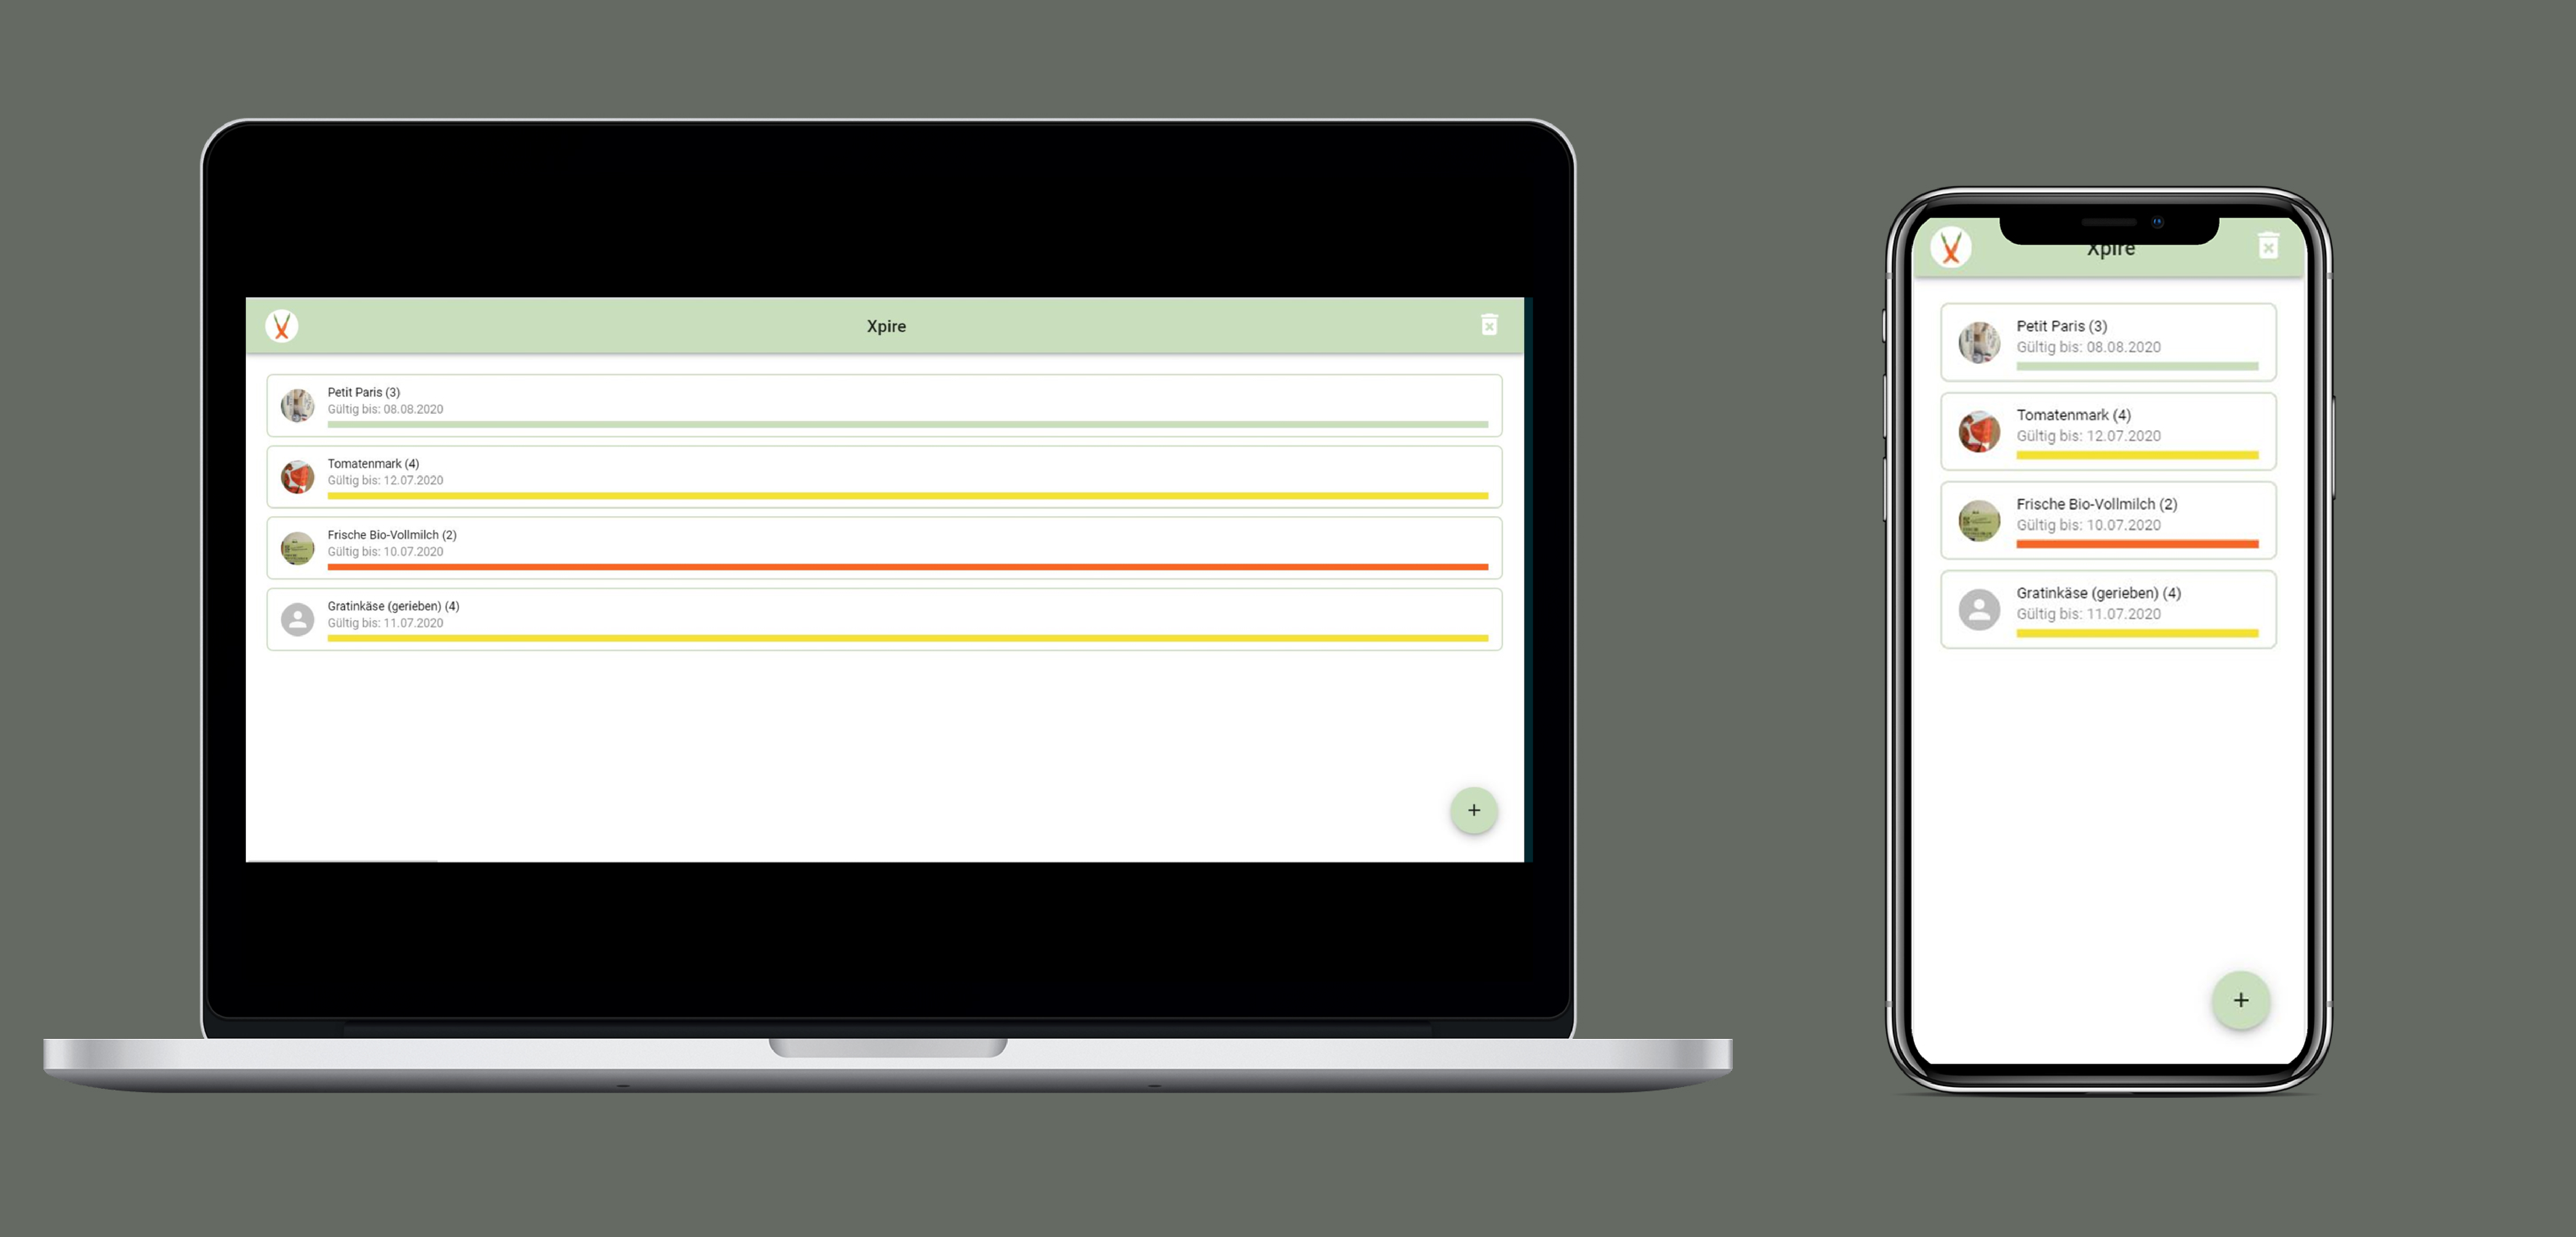
\includegraphics[width=1.0\textwidth]{img/app.pdf}
	\caption{Xpire auf Laptop vs. Smartphone}
	\label{fig:app}
\end{figure}

Die Abbildung \ref{fig:app} zeigt, wie sich die Xpire-App verschiedenen Bildschirmgrößen problemlos anpasst. Zu sehen ist der \textit{Home-Screen} mit eine Auswahl an Beispiel-Produkten.\\



% allgemeine Vorstellung -> Respnsiveness

% Installation

% Tests --> feingarnulare Unit Tests, acceptance tests?

% Deployment